\chapter{Vorgehen}
\label{vorgehen}
Im Rahmen dieses Kapitels wird aufgeführt, wie die Performance-Analyse von Db2 Graph und Neo4j im in Masterarbeit abläuft. Dafür wird zuerst dargelegt, warum es nicht möglich ist, die Messungen und Ergebnisse aus \cite{sigmod_tian} im Rahmen dieser Arbeit zu reproduzieren. Anschließend wird auf die neue Methode für die Performance-Analyse von Db2 Graph und Neo4j eingegangen. 

\section{Reproduktion}
\label{analyse:reproduktion}
Wie in der \nameref{einleitung} aufgeführt, war es in dieser Arbeit vorgesehen, die in \cite{sigmod_tian} erzielten Werte für Db2 Graph zu reproduzieren und mit neuen Werten für Neo4j zu vergleichen. 

Allerdings stellte sich nach einigen Recherchen heraus, dass sich die Werte aus \cite{sigmod_tian} im Rahmen dieser Arbeit nicht reproduzieren lassen. 

Eine Reproduktion der Ergebnisse der Performance-Analyse aus \cite{sigmod_tian} setzt hierbei die folgenden sieben Punkte voraus:
\begin{itemize}
    \item dieselbe Version von Db2 Graph,
    \item dieselbe Db2- und Db2-Graph-Konfiguration,
    \item derselbe Benchmark,
    \item derselbe Db2-Graph-Benchmark-Adapter,
    \item dieselbe Benchmark-Konfiguration,
    \item derselbe Datensatz und 
    \item dieselbe Umgebung (OS, Ressourcen, etc.) wie in \cite{sigmod_tian}.
\end{itemize}
Von diesen sieben Voraussetzungen können im Rahmen der Arbeit jedoch lediglich zwei in einem gewissen Umfang erfüllt werden. Bei diesen zwei Voraussetzungen, die sich teilweise erfüllen lassen, handelt es sich um den Benchmark und die Ressourcen. Die Ressourcen werden hierbei in \cite{sigmod_tian} genau beschrieben. Darüber hinaus wird in \cite{sigmod_tian} auch aufgeführt, dass Linkbench als Benchmark für die Messungen herangezogen wird. Allerdings wird keine Auskunft darüber gegeben, welche Version beziehungsweise Implementierung von Linkbench für die Messungen genutzt wird.

Bezüglich der anderen Punkte werden im Rahmen von \cite{sigmod_tian} keinerlei Informationen bereitgestellt. So ist beispielsweise nicht bekannt, mit welcher Version von Db2 Graph die Messungen durchgeführt wurden. Es ist allerdings wahrscheinlich, dass es sich weder um die Version Beta 3 noch V11.5.6.0 handelt, die über den Zeitraum der Arbeit verfügbar sind. Schließlich wurden beide Versionen mehrere Monate nach der Arbeit veröffentlicht. 

Über die Benchmark-Konfiguration und die Implementierung des für den Benchmark benötigten Db2-Graph-Benchmark-Adapter ist ebenfalls nichts bekannt. Genau so werden in \cite{sigmod_tian} keine Informationen bezüglich der Konfiguration der Db2-Instanz und Db2 Graph angegeben, obwohl diese für die Reproduktion der Ergebnisse eine wichtige Rolle spielen. 

Bezüglich des Datensatzes werden hingegen ein paar Eigenschaften in \cite{sigmod_tian} aufgeführt. Wie und ob der dort verwendet Datensatz durch den Daten-Generator von Linkbench erzeugt werden kann, ist jedoch weiterhin unklar.

\section{Neue Methode}
Da die Reproduktion der Messungen aus \cite{sigmod_tian} nicht möglich ist, muss ein neues Vorgehen für die Analyse der Performance von Db2 Graph und Neo4j definiert werden. Dies erfolgt in diesem Kaptiel. 

Dafür wird zuerst beschrieben, welche Elemente aus \cite{sigmod_tian} in diese Arbeit übernommen werden können. Anschließend wird auf die Änderungen und neuen Aspekte der Performance-Analyse eingegangen. Dabei wird auch begründet, weshalb bestimmte Änderungen vor- und neue Aspekte aufgenommen werden. Als Nächstes wird auf den Aufbau und den Ablauf der Performance-Analyse eingegangen. 

\subsection{Übernommene Elemente}
Auch wenn die Messungen aus \cite{sigmod_tian} nicht reproduziert werden können, so werden trotzdem einige Elemente der Messmethode übernommen, da diese einzelnen Elemente als reproduzierbar und zielführend erachtet werden. Zu diesen Elementen gehören die folgenden Aspekte der Messmethode aus \cite{sigmod_tian}:
\begin{itemize}
    \item Der Einsatz von Linkbench als Benchmark zur Ermittelung der Performance.
    \item Arbeit mit den Datensatzgrößen 10 Millionen und 100 Millionen Knoten (Linkbench-10 und Linkbench-100).
    \item Nutzung der Metriken Latenz und Durchsatz für die Bestimmung der Performance.  
\end{itemize}

\subsection{Änderungen und neue Aspekte}
Die folgenden Aspekte werden neue in die Performance-Analyse mit aufgenommen:
\begin{itemize}
    \item \textit{Db2 Graph Versionen}\\
    Statt, wie in \cite{sigmod_tian} lediglich eine Db2 Graph Version für die Analyse der Performance und den Vergleich mit anderen Graphdatenbanksystemen einzusetzen, werden in dieser Arbeit Beta 3 und V11.5.6.0 beide als Vertreter für Db2 Graph herangezogen. Die beiden Versionen werden dabei in der Performance-Analyse berücksichtigt, da es sich hierbei um die beiden Db2 Graph Versionen handelt, die zum Zeitpunkt des Verfassens der Arbeit verfügbar sind.
    \item \textit{Ergebnismenge}\\
    Im Rahmen der neuen Performance-Analyse soll auch der Einfluss der Größe einer Ergebnismenge einer Anfrage auf die Performance der jeweiligen Datenbanksysteme miteinbezogen werden. Dies wird dabei in die Performance-Analyse mit aufgenommen, da das Verhalten der Datenbanksysteme bei der Abfrage von großen Datenmengen im Kontext dieser Arbeit als relevant eingestuft wird. Wie der Aspekt im Rahmen der Messungen untersucht wird, wird in \autoref{analyse:ergebnismenge} im Detail aufgeführt.
    \item \textit{Verteilung der Datensätze}\\
    Im Rahmen der Performance-Analyse werden nun auch Messungen mit verschieden real und konstant verteilten Datensätzen gemacht. Die Performance der Datenbanksysteme wird hierbei auf Basis von real verteilten Datensätzen ermittelt, um realitätsnahe Ergebnisse zu erlangen. Messungen mit konstant verteilten Datensätzen werden dabei allerdings auch durchgeführt, da es möglich ist, bei diesen auch Ergebnisse für Db2 Graph Beta 3 zu erzielen. Welche Implikationen und Einfluss die Verteilung der Datensätze auf die Messungen der Performance-Analyse hat, wird allerdings in \autoref{analyse:datensatz} genauer erläutert. 
\end{itemize}

\subsection{Ablauf}
Die Performance-Analyse von Db2 Graph und Neo4j, die im Rahmen dieser Arbeit durchgeführt wird, kann in die folgenden Bestandteile unterteilt werden: 
\begin{itemize}
    \item Messung,
    \item Implementierung und 
    \item Auswertung.
\end{itemize}
Die verschiedenen Aspekte, Parameter und Variablen, die bei der Messung eine Rolle spielen, werden dabei in dem nachfolgenden \autoref{messungen} aufgeführt. Darüber hinaus wird hier auch der Aufbau und die Organisation der Messungen in die Messreihe genauer beschrieben. 

Anschließend werden alle für die Durchführung der Performance-Analyse notwendigen Implementierungen in \autoref{implementierung} beschrieben. Dabei wird auf die Wahl der Linkbench-Code-Basis und Umsetzung der Adapter eingegangen. 

Die Auswertung und Präsentation der Ergebnisse erfolgen dann in \compref{ergebnisse} und \compref{auswertung}. In \compref{ergebnisse} wird dabei im Detail auf die Ergebnisse der Messreihen eingegangen, während in \compref{auswertung} eine weiterführende Analyse der Ergebnisse und der Vergleich von Db2 Graph mit Neo4j durchgeführt wird. Darüber hinaus wird in \compref{auswertung} auch versucht, eine Erklärung für den Performance-Unterschied zwischen Db2 Graph Beta 3 und Neo4j zu finden. 

\chapter{Messungen}
\label{messungen}
In diesem Kapitel wird auf die Aspekte, Parameter und Variablen der Messungen eingegangen die bei Performance-Analyse eine Rolle spielen. Hier wird darüber hinaus auch die Konfiguration von Db2 Graph und Neo4j beschrieben, auf deren Basis die Messungen durchgeführt werden. Abschließend wird auf die Gruppierung der Messungen in Messreihen und den Ablauf der Messungen genauer eingegangen.  

\section{Linkbench}
Als Werkzeug zur Messung der Performance wird in der Performance-Analyse der Benchmark Linkbench herangezogen. Aufgrund dessen werden Anpassungen an Linkbench  sowie Linkbench-Adapter für Db2 Graph Beta 3, Db2 Graph V11.5.6.0 und Neo4j benötigt. Die Wahl der Linkbench- und Adapter-Implementierung sowie gegebenenfalls ihre Umsetzungung werden allerdings in \autoref{implementierung} beschrieben. 

In diesem Abschnitt als Teil des Kapitels \nameref{messungen} wird auf die Begriffe: 
\begin{itemize}
    \item Linkbench-Threads,
    \item Request-Anzahl und
    \item Operationsmix eingegangen.
\end{itemize}
Hierbei handelt es sich um wichtige Konfigurationen von Linkbench. Diese spielen während der \textit{Request}-Phase des Benchmarks eine signifikante Rolle. Darüber hinaus stellen sie auch wichtige Parameter für die im Rahmen der Performance-Analyse durchgeführten Messungen dar. 

\subsection{Linkbench-Threads}
\label{analyse:linkbench:threads}
Dabei handelt es sich um eine Einstellung des Benchmarks, die in der Adapter-Konfiguration von Linkbench erfolgt. Innerhalb der Konfiguration wird sie auch durch den Key \texttt{requesters} gesetzt. 

Im Rahmen der Arbeit wird die Konfiguration allerdings als Linkbench-Threads bezeichnet, da durch diese spezifiziert wird, wie viele Threads während des Benchmarks gleichzeitig Requests beziehungsweise Graph-Queries an ein Datenbanksystem senden.

Es handelt sich somit um eine Einstellung, die einen erheblichen Einfluss auf die bei der Performance-Analyse erzielten Ergebnisse hat. Schließlich hat die Anzahl der Threads, die gleichzeitig während den Messungen Anfragen an ein Datenbanksystem senden, einen großen Einfluss darauf, welche Last während des Benchmarks auf ein Datenbanksystem ausgeübt wird. 

Bei den Linkbench-Threads handelt es sich darüber hinaus um einen Parameter, der über alle Messreihen der Arbeit hinweg konstant den Wert 50 aufweist. So kann sichergestellt werden, dass während den Messungen alle Datenbanksysteme zumindest in dieser Hinsicht derselben Last ausgesetzt sind. 

\subsection{Request-Anzahl}
\label{analyse:request_anzahl}
Bei der Request-Anzahl handelt es sich, wie bei den Linkbench-Threads, ebenfalls um eine Einstellung, die in der Adapter-Konfiguration von Linkbench vorgenommen wird. Um sie festzulegen, muss ein Wert für \texttt{requests} angegeben werden. 

Zum besseren Verständnis wird die Konfiguration allerdings im weiteren Verlauf als Request-Anzahl bezeichnet. Die Request-Anzahl regelt dabei, wie viele Graph-Queries von jeweils einem der Linkbench-Threads an das zu benchmarkende Datenbanksystem gesendet werden, bevor eine \textit{Request}-Phase endet und die Ergebnisstatistik (eine CSV-Datei) erstellt. Der Faktor wirkt sich dadurch signifikant darauf aus, wie lange eine \textit{Request-Phase} andauert, bevor Linkbench die Ergebnisse für das untersuchte Datenbanksystem in Form einer Ergebnisstatistik bereitstellt. Zugleich bietet er einen Anhaltspunkt für die Qualität der durchgeführten Messungen. Denn Linkbench erhält ein umso detaillierteres Bild von der Performance der Datenbanksysteme, desto mehr Requests beziehungsweise Graph-Queries Teil des Benchmark-Durchlaufs sind. Darüber hinaus fallen bei einer höheren Anzahl an Messungen auch Anomalien weniger ins Gewicht, welche die Messergebnisse gegebenenfalls verzerren könnten.

Im Rahmen der in der Arbeit durchgeführten Messreihen muss hierbei ein Kompromiss zwischen der Qualität und der Dauer einer \textit{Request}-Phase von Linkbench gefunden werden. 

So wird bei allen Messungen, die auf Basis eines konstant verteilten Datensatzes durchgeführt werden, die Request-Anzahl von 500.000 eingesetzt. Diese Anzahl wird dabei gewählt, da sie ein detailliertes Bild von der Performance eines Datenbanksystems zeichnet und sich die \textit{Request}-Phase für alle drei Datenbanksysteme unterhalb eines Zeitraums von drei Stunden befindet -- sollte es zu keinen Anomalien kommen. 

Für die Messungen, die auf Basis eines real verteilten Datensatzes erfolgen, wird lediglich eine Request-Anzahl von 50.000 herangezogen. Dies hängt damit zusammen, dass hierbei deutlich umfangreichere Ergebnismengen möglich sind. So kann es je nach Variation der \texttt{getLinkList}-Ope\-ra\-ti\-on, zu einer Ergebnismenge von bis zu 100.000 Links (Kanten) kommen. Eine solch große Ergebnismenge hat einen signifikanten Einfluss auf die Performance der Datenbanksysteme während des Benchmarks. Dies kann zur Folge haben, dass die Performance eines Datenbanksystems nachweisbar einbricht. Um weiterhin eine Performance von unter drei Stunden für eine Request-Phase gewährleisten zu können, wird die Request-Anzahl daher reduziert. Auch wenn dadurch nicht dieselbe Qualität der Ergebnisse erreicht werden kann, wie bei den Messungen mit einem konstant verteilten Datensatz.

Die unterschiedliche Request-Anzahl bei den verschiedenen Messreihen stellt einen wichtigen Punkt dar, der später bei dem Vergleich der Ergebnisse miteinander beachtet werden muss. Schließlich fällt beispielsweise bei Messungen mit einer geringeren Request-Anzahl die Anfangsphase, in der die Datenbanksysteme oft erst warmlaufen, stärker ins Gewicht als bei Messungen mit einer höheren Request-Anzahl.

\subsection{Operationsmix}
\label{analyse:linkbench:operationsmix}
Beim Operationsmix handelt es sich um Einstellungen, die in der Workload-Konfiguration von Linkbench vorgenommen werden. Sie bestimmen dabei, welchen Anteil eine Operation an der Gesamtzahl von Requests während der \textit{Request}-Phase hat. Wird beispielsweise in der Workload-Konfiguration der Parameter \texttt{getnode} auf 100 gesetzt, so handelt es sich bei allen Operationen, die während einer \textit{Request}-Phase durchgeführt werden, um \texttt{getNode}-Operationen.

Im Rahmen der Arbeit wird die Zusammensetzung des Operationsmix dabei immer zwischen allen Messungen eines Datenbanksystems in einer bestimmten Konfiguration variiert. Dabei macht eine Operation beziehungsweise Operationsart immer 100 \% aller im Rahmen einer Messung durchgeführten Requests aus. So wird jede Operationsart wie \texttt{getNode}, \texttt{getLink}, etc. im Rahmen einer separaten \textit{Request}-Phase von Linkbench gemessen und analysiert.

Die Operationen werden getrennt voneinander gemessen, um die während der \textit{Request}-Phase erzielte Ressourcenauslastung immer einer bestimmten Operationsart zuordnen zu können. Wie die Ressourcenauslastung gemessen wird, wird in \autoref{analyse:metriken} genauer beschrieben.

\section{Operationen}
\label{analyse:operationen}
In diesem Abschnitt wird auf die verschiedenen Operationen eingegangen, deren Performance im Rahmen der Analyse dieser Arbeit eine Rolle spielen. 

Bei den im Rahmen der Performance-Analyse gebenchmarkten Operationen handelt es sich um dieselben Operationen, die auch in \cite{sigmod_tian} untersucht werden. Es gilt allerdings zu beachten, dass obwohl die Namen der Operationen gleich lauten, nicht bekannt ist, ob die Queries, die von ihnen an die Datenbanksysteme gesendet werden, identisch sind. Daher sollten aus den gleichen Namen keine falschen Schlüsse gezogen werden. 

Des Weiteren ist es auch nicht möglich, die untersuchten Operationen im Vergleich zu \cite{sigmod_tian} auszuweiten. Schließlich handelt es sich bei diesen um lesende Operationen, die dadurch auch von Db2 Graph als eine Art Read-Only-Datenbanksystem unterstützt werden. Alle weiteren Operationen, die von Linkbench bereitgestellt werden (\autoref{linkbench:operationen}), sind hingegen von schreibender Natur. 

Bei den im Rahmen der Performance-Analyse gebenchmarkten Operationen handelt es sich um:
\begin{itemize}
    \item \texttt{getNode},
    \item \texttt{getLink},
    \item \texttt{countLink} und
    \item \texttt{getLinkList}. 
\end{itemize}

Wobei es allerdings anzumerken gilt, dass bei den Messungen mit Bezug zu real verteilten Datensätzen vier verschiedene Varianten von \texttt{getLinkList} gemessen werden. Bei diesen Varianten variiert jeweils die maximale Größe der sogenannten Ergebnismenge. Dies führt dazu, dass in der Praxis eigentlich die folgenden sieben Operation gebenchmarkt werden:
\begin{itemize}
    \item \texttt{getNode},
    \item \texttt{getLink},
    \item \texttt{countLink},
    \item \texttt{getLinkList(100)},
    \item \texttt{getLinkList(1.000)},
    \item \texttt{getLinkList(10.000)} und
    \item \texttt{getLinkList(100.000)}.
\end{itemize}
Die eingeklammerten Zahlen bei \texttt{getLinkList} repräsentieren hierbei die obere Grenze der Ergebnismenge der Operation. Die Rolle und der Einsatz der Begrenzung der Ergebnismenge wird dabei im nächsten Abschnitt \autoref{analyse:ergebnismenge} im Detail erläutert. 

\section{Begrenzung der Ergebnismenge}
\label{analyse:ergebnismenge}
In diesem Abschnitt wird auf die Rolle der Begrenzung der Ergebnismenge bei der \texttt{getLinkList}-Ope\-ra\-ti\-on genauer eingegangen. Diese spielt im Kontext der Performance-Analyse eine wichtige Rolle, da sie bei einigen Messungen eine signifikante Stellung als Messparameter einnimmt, welche es bei der Auswertung der Ergebnisse zu beachten gilt. 

Bei der Begrenzung der Ergebnismenge handelt es sich um eine Workload-Konfiguration, die lediglich die \texttt{getLinkList}-Ope\-ra\-ti\-on betrifft. Durch sie wird eine obere Grenze für die Anzahl an Elementen einer Ergebnismenge in der Query der \texttt{getLinkList}-Ope\-ra\-ti\-on gesetzt. Wird die Grenze beispielsweise auf 10 gesetzt, so übermitteln die abgefragten Datenbanksysteme als Antwort auf die \texttt{getLinkList}-Queries maximal eine Menge mit zehn Links (Kanten) an den Benchmark. 

Die Begrenzung der Ergebnismenge wird im Rahmen dieser Arbeit auch kurz als Range-Limit bezeichnet, da der Key \texttt{range\_limit} in der Workload-Konfiguration für die Steuerung der Begrenzung der Ergebnismenge verantwortlich ist. 

Sie wird in den Benchmark eingeführt, um die Performance der verschiedenen Datenbanksysteme bei größeren oder kleineren Ergebnismengen untersuchen zu können.

Bei den Messungen, die im Rahmen dieser Arbeit durchgeführt werden, nimmt die obere Grenze der Ergebnismenge die folgenden Werte an:
\begin{itemize}
    \item 100,
    \item 1.000,
    \item 10.000 und
    \item 100.000. 
\end{itemize}
Diese werden dabei ausgewählt, da der Faktor-10-Unterschied zwischen den Werten für eine Differenz sorgt, von der angenommen wird, dass sie ausreicht, um aussagekräftige Messergebnisse für die \texttt{getLinkList}-Ope\-ra\-ti\-on zu erzielen. 

100.000 wird darüber hinaus als größte Menge gewählt, da eine Grenze von 1.000.000 zur Folge hätte, das der Messzeitraum der \texttt{Request}-Phase von 3 Stunden bei einigen Messungen um ein Vielfaches überschritten worden wäre.

Wie bereits zuvor erwähnt, spielt die Variation der Begrenzung der Ergebnismenge lediglich bei den Messungen mit Bezug zu real verteilten Datensätzen eine Rolle. Dies hängt damit zusammen, dass bei konstant verteilten Datensätzen im Rahmen dieser Arbeit immer eine sogenannte 10er-Verteilung vorherrscht. Was bedeutet, dass die Ergebnismenge für die \texttt{getLinkList}-Ope\-ra\-ti\-on maximal 10 Elemente beinhalten kann, egal ob die obere Grenze für die Größe der Ergebnismenge 100 oder 100.000 beträgt. Somit erübrigt sich die Variation der Begrenzung der Ergebnismenge bei diesen Messungen. 

\section{Queries}
\label{analyse:queries}
Dieser Abschnitt setzt sich mit den Gremlin- und Cypher-Queries auseinander, die für die Umsetzung der Messungen herangezogen werden. Es gilt hierbei darauf hinzuweisen, dass die in diesem Abschnitt dargestellten Queries in gewissem Ausmaß der Implementierung der Adapter in \autoref{implementierung} vorgreift. Allerdings nehmen die Queries eine signifikante Rolle bei den Messungen ein. Schließlich handelt es sich bei ihnen um die Anfragen, die im Zuge der Durchführung einer Operation während des Benchmarks zur Interaktion mit den Datenbanksystemen herangezogen wird. Daher werden sie bereits in diesem Abschnitt näher beschrieben.

Wie zuvor erwähnt, kann bei diesen Anfragen zwischen Gremlin- und Cypher-Queries unterschieden werden. Die in der Abfragesprache Gremlin formulierten Queries werden dabei in \autoref{src:gremlin_queries} aufgeführt, während \autoref{src:cypher_queries} die in Cypher umgesetzten Queries abgebildet. Im Zuge dessen gilt es darauf hinzuweisen, dass in \autoref{src:gremlin_queries} Platzhalter innerhalb der Queries von \texttt{<} und \texttt{>} umschlossen werden. Bei \autoref{src:cypher_queries} werden sie hingegen mittels eines anführenden \texttt{\$} gekennzeichnet.

Die Gremlin- und Cypher-Queries, welche im \autoref{src:gremlin_queries} und \autoref{src:cypher_queries} aufgeführt werden verfügen darüber hinaus über dieselbe Abfragelogik. Damit ist gemeint, dass beide dieselben Daten abfragen, wodurch sie äquivalent zueinander sind. Die Gremlin-Queries werden dabei zur Abfrage von Db2 Graph Beta 3 und V11.5.6.0 genutzt, während die Cypher-Queries für Neo4j zum Einsatz kommen. 

\begin{lstlisting}[label=src:gremlin_queries,caption={Gremlin-Queries},language=Java]
/* getNode */
g.V()
 .hasLabel("NODETABLE")
 .has("ID", <NODE_ID>);

/* getLink */
g.E()
 .hasLabel("LINKTABLE")
 .has("LINK_TYPE", <LINK_TYPE>)
 .has("ID1", <NODE_ID1>)
 .has("ID2", P.within(<NODE_ID2s>))

/* countLink */
g.V()
 .hasLabel("NODETABLE")
 .has("ID", <NODE_ID>)
 .outE("LINKTABLE")
 .has("LINK_TYPE", <LINK_TYPE>)
 .count()

/* getLinkList */
g.V()
 .hasLabel("NODETABLE")
 .has("ID", <NODE_ID1>)
 .outE("LINKTABLE")
 .has("LINK_TYPE", <LINK_TYPE>)
 .limit(<LIMIT>);
\end{lstlisting}

\begin{lstlisting}[label=src:cypher_queries,caption={Cypher-Queries},language=CQL]
/* getNode */
MATCH (n:node{id: $id}) 
RETURN n.id AS ID, n.type AS TYPE, 
    n.version AS VERSION, n.time AS TIME, 
    n.data AS DATA

/* getLink */
MATCH (n1:node{id: $id1})-[l:link{link_type: $link_type}]->(n2:node) 
WHERE n2.id IN $id2s 
RETURN n1.id AS ID1, n2.id AS ID2, 
    l.link_type AS LINK_TYPE, 
    l.visibility AS VISIBILITY, 
    l.data AS DATA, l.time AS TIME, 
    l.version AS VERSION

/* countLink */
MATCH (:node{id: $id1})-
    [l:link{link_type: $link_type}]->
    (:node) 
RETURN COUNT(l) AS COUNT

/* getLinkList */
MATCH (n1:node{id: $id1})-
    [l:link{link_type: $link_type}]->
    (n2:node) 
RETURN n1.id AS ID1, n2.id AS ID2, 
    l.link_type AS LINK_TYPE, 
    l.visibility AS VISIBILITY, 
    l.data AS DATA, l.time AS TIME, 
    l.version AS VERSION 
LIMIT $limit
\end{lstlisting}

\section{Datensatz}
\label{analyse:datensatz}
Die Zusammensetzung des Datensatzes und ihre Verteilung spielen infolge der neuen Zielsetzung der Arbeit eine zentrale Rolle für die Performance-Analyse der Dateisysteme.

In diesem Abschnitt wird daher zuerst auf die beiden Arten der Verteilung der Datensätze eingegangen. Im Anschluss daran wird der Aspekt der Größe eines Datensatzes genauer beleuchtet.

\subsection{Verteilung}
Im Rahmen der Arbeit wird zwischen den beiden folgenden Arten der Verteilung unterschieden:
\begin{itemize}
    \item \textit{konstante Verteilung}\\
    Hierbei besitzt jeder Knoten im Datensatz exakt dieselbe Anzahl an Kanten (Links) wie jeder andere Knoten. Im Rahmen dieser Arbeit wird bei allen Messungen immer eine konstante 10er-Verteilung gewählt. Dies bedeutet, dass jeder Knoten genau 10 Kanten aufweist. 
    \item \textit{reale Verteilung}\\
    Dabei ist die Verteilung von Kanten (Links) auf Knoten einer realen Verteilung eines Social-Graphs nachempfunden. Die Anzahl der Kanten, über die ein Knoten verfügt, bewegt sich hierfür bei allen Messungen, die in dieser Arbeit durchgeführt werden, zwischen 2 und ca. 5.000.000. Dabei existieren allerdings viele Knoten mit einer kleinen Anzahl an ausgehenden Kanten, während dem lediglich eine überschaubare Menge an Knoten über mehr als 1.000.000 Kanten verfügt.
\end{itemize}
Die real-Verteilung wird hierbei im Zuge der Performance-Analyse untersucht, da sie die realitätsnahe Zusammensetzung eines Social-Graphs aufweist. Somit geben die Messergebnisse einen Einblick, wie sich die Datenbanksysteme bei solchen Workloads in der Praxis verhalten könnten.

Die konstante Verteilung wird entgegen der real-Verteilung nicht aufgrund ihrer Praxisnähe für die Messungen herangezogen. Sie wird stattdessen eingeführt, da Db2 Graph Beta 3 bei ersten Messungen Schwierigkeiten mit einer hohen Kantenzahl in real verteilten Datensätzen aufwies. Das Benchmarking der \texttt{getLinkList}-Ope\-ra\-ti\-on verursachte dabei früher oder später einen beinahe Stillstand des Benchmark-Durchlaufs. 

Dieses Verhalten kann dadurch begründet werden, dass sich Db2 Graph Beta 3 damit schwertut, mit großen Ergebnismengen von über 100.000 Kanten je Knoten zu arbeiten. Darüber hinaus kann dieses Problem von Db2 Graph Beta 3 mit real verteilten Datensätzen auch nicht durch die Begrenzung der Ergebnismenge im Rahmen der Gremlin-Query gelöst werden. Schließlich beherrscht Db2 Graph Beta 3 die Optimierung \textit{Limit Pushdown} nicht, siehe \autoref{db2graph:optimierung}. 

Aufgrund dessen und da es -- nachvollziehbarerweise -- nicht zielführend wäre, die maximale Kanten auf Knoten Verteilung eines real verteilten Datensatzes zu verändern, werden auch Szenarien mit konstant verteilten Datensätzen in die Arbeit aufgenommen. Schließlich ergibt sich dadurch die Möglichkeit, Messergebnisse für Db2 Graph Beta 3 zu erzielen und diese mit V11.5.6.0 und Neo4j zu vergleichen. Allerdings nur unter der Voraussetzung, dass eine kleine konstante Verteilung, wie die konstante 10er-Verteilung, gewählt wird. 

Aufgrund des zuvor angesprochenen Problems von Db2 Graph Beta 3 mit real verteilten Datensätzen spielt Beta 3 auch bei den Messungen, die auf real verteilten Datensätzen aufbauen, im Kontext dieser Arbeit keine Rolle. Was bedeutet, dass bei diesen keinerlei Messungen mit Beta 3 durchgeführt werden, lediglich mit Db2 Graph V11.5.6.0 und Neo4j. 

\subsection{Größe}
Die Größe eines Datensatzes stellt neben dessen Verteilung einen großen Unterschied zwischen den im Rahmen der Performance-Analyse durchzuführenden Messungen dar. Dabei wird hier unter der neuen Zielsetzung der Arbeit ebenfalls mit den aus \cite{sigmod_tian} bekannten Begriffen Linkbench-10M und Linkbench-100M gearbeitet. Die Begriffe beschreiben hierbei grob eine Datensatzgröße. So stehen die 10M und 100M jeweils dafür, dass ein Datensatz jeweils 10 oder 100 Millionen Knoten beinhaltet. Die Linkbench-10M Datensätze stellen dadurch die kleineren Datensätze im Rahmen der Performance-Analyse dar, während die Linkbench-100M Datensätze die Rolle des größeren Datensatzes einnehmen. 

Die Variation der Datensatzgröße über die im Rahmen der Performance-Analyse durchgeführten Messungen stellt dabei einen interessanten Untersuchungsaspekt dar. Schließlich gilt es bei der Beurteilung von Datenbanksystemen immer zu beachten, wie diese mit kleineren oder größeren Datenmengen umgehen.

Bei den Begriffen Linkbench-10M und Linkbench-100M muss allerdings darauf aufmerksam gemacht werden, dass sich die Datensätze je nach Verteilung weiterhin in ihrer Größe unterscheiden können. So verfügen ein real verteilter und ein konstant verteilter Linkbench-10M Datensatz im Rahmen der Arbeit immer über unterschiedliche Größen. Dies hängt damit zusammen, dass sie aufgrund der Verteilung eine unterschiedliche Anzahl an Kanten beinhalten, auch wenn sie gleich viele Knoten besitzen. So weisen die konstant verteilten Datensätze aus \autoref{tab:kanten_anzahl} fast die doppelte Anzahl an Kanten auf, wie die real verteilten Datensätze. 

\begin{table}[ht]
    \centering
    \begin{tabular}{l|r|r}
    \hline
    \rowcolor[HTML]{EFEFEF} 
    \multicolumn{1}{c|}{\cellcolor[HTML]{EFEFEF}\textbf{Verteilung}} & \multicolumn{1}{c|}{\cellcolor[HTML]{EFEFEF}\textbf{Linkbench-10M}} & \multicolumn{1}{c}{\cellcolor[HTML]{EFEFEF}\textbf{Linkbench-100M}} \\ \hline
    real & ca. 53.000.000 Kanten & ca. 530.000.000 Kanten \\
    konstant & 100.000.000 Kanten & 1.000.000.000 Kanten \\ \hline
    \end{tabular}
    \caption{Übersicht Linkbench Kantenanzahl}
    \label{tab:kanten_anzahl}
\end{table}

Aufgrund dessen sollte auch später vom Vergleich der Messergebnisse zwischen den unterschiedlich verteilten Datensätzen bei Linkbench-10M und Linkbench-100M abgesehen oder aufgepasst werden.

\section{Metriken}
\label{analyse:metriken}
Bei den Messungen, die im Rahmen der Arbeit durchgeführt werden, werden wie bereits in \cite{sigmod_tian} thematisiert, die Metriken Latenz und Durchsatz für die Auswertung der Ergebnisse herangezogen. Die Beiden stellen hierbei die Metriken dar, anhand derer die Performance von Db2 Graph und Neo4j in dieser Arbeit gemessen, beurteilt und verglichen wird.

Der Begriff Latenz bezeichnet dabei den Zeitraum zwischen dem Abschicken einer Anfrage an ein Datenbanksystem und dem Eintreffen der Antwort auf die Anfrage. Alternative kann die Latenz auch als Verarbeitungszeit, also die Zeit, die ein Datenbanksystem für die Verarbeitung einer Anfrage benötigt, betrachtet werden. Die Latenzwerte, die im weiteren Verlauf dieser Arbeit aufgeführt und dargestellt werden, werden dabei alle den Ergebnisstatistiken entnommen, die nach Abschluss einer mit Linkbench durchgeführten Messung erzeugt werden. 

Unter der Metrik Durchsatz wird während der Performance-Analyse erfasst, wie viele Operationen pro Sekunde durchschnittlich während einer Messung durchgeführt werden konnten. Die Durchsatzwerte, die im Kontext dieser Arbeit dargelegt werden, stammen alle aus den letzten Zeilen der Log-Dateien, die von Linkbench im Zuge der Messungen erzeugt werden.

Darüber hinaus werden während allen Messungen Ressourcenstatistiken erfasst. Diese Statistiken werden dabei von dem Werkzeug NMON erstellt. Während einer Messung zeichnet dieses einmal pro Minute  einen Datenpunkt auf. Diese Statistiken geben einem dabei einen Einblick darüber, wie groß der Ressourcenverbrauch der Datenbanksysteme während der Messungen ist.

\section{Umgebung}
\label{analyse:umgebung}
Für alle Messungen, die Teil der Performance-Analyse sind, wird im Rahmen der Arbeit derselbe Server herangezogen. Bei diesem handelt es sich um einen Ubuntu-Server 20.04.2 LTS mit folgenden Charakteristika:
\begin{itemize}
    \item 32 CPUs (AMD EPYC 7502P), 
    \item 256 GB Arbeitsspeicher,
    \item 500 GB SSD-Hauptspeicher,
    \item \texttt{ext4} als Dateisystem und 
    \item dem Linux-Kernel \texttt{5.4.0-77-generic}.
\end{itemize}
Des Weiteren gilt es herauszustellen, dass die folgenden Datenbanksysteme während Messungen alle als Docker-Container betrieben werden: 
\begin{itemize}
    \item Db2,
    \item Db2 Graph Beta 3,
    \item Db2 Graph V11.5.6.0 und 
    \item Neo4j. 
\end{itemize}
Jedes dieser Systeme wird dabei in einem eigenen Container betrieben. 

\section{Datenbanksysteme}
\label{analyse:datanbanksysteme}
Im Rahmen der Performance-Analyse werden Messungen mit den folgenden Datenbanksystemen durchgeführt: 
\begin{itemize}
    \item Db2 Graph Beta 3 (+ Db2),
    \item Db2 Graph V11.5.6.0 (+ Db2) und
    \item Neo4j.
\end{itemize}
In den folgenden Unterabschnitten werden dabei die wichtige Anwendungs- beziehungsweise System-Konfigurationen beschrieben. 

\subsection{Db2}
Die beiden Db2 Graph Versionen verwenden bei allen Messungen Performance-Analyse dieselbe Db2-Instanz. Dadurch wird gewährleistet, dass beide auf ein relationales Datenbankmanagementsystem zugreifen, das sich nicht in der Konfiguration zwischen den Db2 Graph Versionen unterscheidet. Außerdem können somit beide Db2 Graph Versionen auf Basis eines identischen Datensatzes operieren. Auf diese Weise kann eine Verzerrung der Messergebnisse vermieden werden, sodass beide Versionen von Db2 Graph während des Benchmarks unter denselben Voraussetzungen arbeiten können.

Bei der Db2-Instanz, die von beiden Db2 Graph Versionen genutzt wird, handelt es sich um die Db2 Advanced Edition in Version V11.5.5.1. Per Konfiguration wird ihr 180 GB an Arbeitsspeicher zugewiesen. Darüber hinaus verfügt sie über die für Linkbench benötigte Datenbank \texttt{linkdb0}. Diese weist im Kontext aller Messungen das in \autoref{src:linkdb0_schema} beschrieben Datenbankschema auf:

\begin{lstlisting}[label=src:linkdb0_schema,caption={Db2-Instanz Datenbankschema für linkdb0},language=SQL]
CREATE TABLE linkdb0.nodetable
(
    id      bigint NOT NULL GENERATED ALWAYS AS IDENTITY (START WITH 1 INCREMENT BY 1),
    type    int       NOT NULL,
    version numeric   NOT NULL,
    time    int       NOT NULL,
    data    clob(48000)  NOT NULL,
    PRIMARY KEY (id)
) ORGANIZE BY ROW COMPRESS YES;

CREATE TABLE linkdb0.linktable
(
    id1        bigint  NOT NULL DEFAULT '0',
    id2        bigint  NOT NULL DEFAULT '0',
    link_type  bigint  NOT NULL DEFAULT '0',
    visibility smallint     NOT NULL DEFAULT '0',
    data       varchar(255) NOT NULL DEFAULT '',
    time       bigint  NOT NULL DEFAULT '0',
    version    bigint       NOT NULL DEFAULT '0',
    PRIMARY KEY (link_type, id1, id2)
) ORGANIZE BY ROW COMPRESS YES;

/* Exisitiert, wird aber nicht genutzt. */
CREATE TABLE linkdb0.counttable
(
    id        bigint NOT NULL DEFAULT '0',
    link_type bigint NOT NULL DEFAULT '0',
    count     int         NOT NULL DEFAULT '0',
    time      bigint NOT NULL DEFAULT '0',
    version   bigint NOT NULL DEFAULT '0',
    PRIMARY KEY (id, link_type)
) ORGANIZE BY ROW COMPRESS YES;
\end{lstlisting}

An dem in \autoref{src:linkdb0_schema} beschriebenen Schema kann dabei abgelesen werden, dass alle Tabellen adaptive Kompression nutzen. Außerdem existiert in \autoref{src:linkdb0_schema} eine Count-Tabelle (\texttt{linkdb0.counttable}) die von den Linkbench-Adaptern für Db2 Graph Beta 3 und V11.5.6.0 nicht genutzt wird. Sie ist lediglich vorhanden, da Linkbench ihre Existenz voraussetzt. 

Neben dem Datenbankschema von \texttt{linkdb0} muss auch noch darauf hingewiesen werden, dass die Datenbank einen Bufferpool (\texttt{IBMDEFAULTBP}) der Größe 163,920 GB nutzt. Der Bufferpool besteht dabei aus exakt 40.000.000 Seiten, mit einer Seitengröße (\texttt{PAGESIZE}) von 4096 Byte.

\subsection{Db2 Graph}
Die Version Beta 3 und V11.5.6.0 von Db2 Graph verfügen im Rahmen der Performance-Analyse über eine vergleichbare Konfiguration. Lediglich die in V11.5.6.0 neu eingeführten \texttt{db2graph-server.yaml} und \texttt{db2graph-internal.ya\allowbreak ml} sorgen dafür, dass es Konfigurationsunterschiede zwischen beiden Versionen gibt. Auf diese beiden Konfigurationen wird allerdings nicht näher eingegangen. Schließlich werden die beiden Konfigurationen nicht für die Messungen angepasst. Somit zieht Db2 Graph V11.5.6.0 bei allen Messungen im Zuge der Performance-Analyse die Standard-Konfiguration von \texttt{db2graph-server.yaml} und \texttt{db2graph-internal.yaml} heran, welche mit dem jeweiligen Container-Image ausgeliefert wird.

Für die Messungen werden die Konfiguration \texttt{gremlin-server.yaml} sowie die Ressourcenparameter des Gremlin-Servers beider Versionen gleichermaßen angepasst. Bei diesen Anpassungen handelt es sich um:
\begin{itemize}
    \item \textit{Gremlin-Memory}\\
    Dieser Ressourcenparameter legt fest, wie viel Memory der Gremlin-Server des TinkerPop-Stacks im Maximalfall nutzen kann. Der Standard-Wert beträgt bei beiden Db2 Graph Versionen normalerweise 4 GB. Um eine möglichst hohe Performance mit beiden Db2 Graph Versionen zu erzielen, wird das Memory-Limit für den Gremlin-Server im Rahmen der Messungen allerdings auf 64 GB angehoben. 
    \item \textit{Thread-Pool-Worker}\\
    Der Wert für Thread-Pool-Worker regelt, wie viele Threads für die Verarbeitung von nicht-blockenden Operationen im Gremlin-Server bereitstehen \cite{tinkerpop_2020}. Der Wert ist dabei normalerweise auf 0 gesetzt, was zur Folge hat, dass die Anzahl von verfügbaren Prozessoren herangezogen wird \cite{tinkerpop_2020}. Dies hätte im Kontext der Messumgebung zur Folge, dass die Thread-Pool-Worker standardmäßig auf 32 gesetzt werden würden. 
    
    Um eine möglichst hohe Performance für die Db2 Graph Versionen bei den Messungen zu gewährleisten, wird der Wert allerdings auf 128 erhöht. Dadurch unterstützt es den Gremlin-Server dahingehend, große Lasten besser zu verarbeiten. Dadurch ist es ihm möglich, 50 oder 100 Anfragen, die von den entsprechenden Linkbench-Threads während des Benchmarkings gesendet werden, auf einmal zu bearbeiten. 
    \item \textit{Gremlin-Pool}\\
    Der Wert für den Gremlin-Pool spezifiziert, wie viele Threads dem Gremlin-Server für die Verarbeitung von blockenden Operationen zur Verfügung stehen \cite{tinkerpop_2020}. Ähnlich wie Thread-Pool-Worker zieht er in der Standard-Konfiguration die verfügbare Prozessoranzahl (32) heran \cite{tinkerpop_2020}. Um eine höhere Performance zu erreichen, wird er allerdings ebenfalls auf 128 erhöht. 
    
    Die Erhöhung wird hierbei als Vorsichtsmaßnahme durchgeführt. Schließlich unterstützt Db2 Graph ausschließlich lesende Queries. Dies hat zur Folge, dass der Gremlin-Server eigentlich nicht auf blockende Operationen zurückgreifen sollte. Allerdings ist nicht bekannt, ob Db2 Graph in der Praxis wirklich nur auf nicht-blockende Operationen zurückgreift. Daher wird der Wert des Gremlin-Pools analog zu Thread-Pool-Worker angehoben. 
\end{itemize}

Beide Versionen von Db2 Graph nutzen darüber hinaus die in \autoref{src:db2graph_mapping} dargestellte Graph-Overlay-Konfiguration, zum Mapping der in \autoref{src:linkdb0_schema} beschrieben Tabellen auf eine Graphstruktur. Hierbei wird die \texttt{linkdb0.nodetable} aus \autoref{src:linkdb0_schema} als Vertex-Tabelle in \autoref{src:db2graph_mapping} herangezogen, während die \texttt{linkdb0.linktable} die Rolle einer Edge-Tabelle übernimmt. 
\begin{lstlisting}[label=src:db2graph_mapping,caption={Graph-Overlay-Konfiguration Db2 Graph},language=json]
...
"jdbc_num_conn": 100,
"v_tables": [
    {
        "vid": {
            "prefix": "LINKDB0.NODETABLE",
            "id_cols": [
                "ID"
            ]
        },
        "table_id": "LINKDB0.NODETABLE",
        "table": {
            "schema_name": "LINKDB0",
            "table_name": "NODETABLE"
        },
        "label": {
            "fixed_label": true,
            "label": "NODETABLE"
        }
    }
],
"e_tables": [
    {
        "src_v_cols": [
            "ID1"
        ],
        "dst_v_cols": [
            "ID2"
        ],
        "src_v_tables": [
            "LINKDB0.NODETABLE"
        ],
        "dst_v_tables": [
            "LINKDB0.NODETABLE"
        ],
        "eid": {
            "implicit_id": false,
            "id": {
                "prefix": "LINKDB0.LINKTABLE",
                "id_cols": [
                    "LINK_TYPE",
                    "ID1",
                    "ID2"
                ]
            }
        },
        "table_id": "LINKDB0.LINKTABLE",
        "table": {
            "schema_name": "LINKDB0",
            "table_name": "LINKTABLE"
        },
        "label": {
            "fixed_label": true,
            "label": "LINKTABLE"
        }
    }
]
\end{lstlisting}

\subsection{Neo4j}
Alle Messungen, die im Rahmen der Performance-Analyse durchgeführt werden, nutzen dieselbe Neo4j-Instanz. Bei dieser Instanz handelt es sich um die Community-Edition von Neo4j in Version 4.3. An der Konfiguration von Neo4j ändert sich zwischen den verschiedenen Messreihen nichts. Sie weist somit immer dieselbe Konfiguration auf. Bei dieser Konfiguration gilt es die folgenden Parameter hervorzuheben: 
\begin{itemize}
    \item 160 GB Page Cache und
    \item maximaler JVM Heap 64 GB.
\end{itemize}
Der Page Cache kann dabei als das Neo4j-Pendant zum Bufferpool von Db2 betrachtet werden. Daher wird mit ca. 164 GB und 160 GB auch eine vergleichbare Konfiguration für beide gewählt. Der JVM Heap in Neo4j und der Gremlin-Memory von Db2 Graph werden hierbei aufgrund ihrer ähnlichen Funktion ebenfalls als vergleichbar angesehen, weshalb beide auf 64 GB gesetzt werden.

Bei Neo4j handelt es sich um eine native Graphdatenbank, die auf dem in \autoref{datenmodelle} beschrieben Graphmodell basiert. Dadurch unterstützt Neo4j ein flexibles Datenbankschema, wie in \autoref{datenmodelle:structure} bereits beschrieben. Neo4j unterstützt allerdings trotz des flexiblen Schemas die Definition von Constraints. Ein solcher Constraint und ein Index werden in den Graphdatenbank eingerichtet, um einen fairen Vergleich zwischen den Db2graph Versionen (+ Db2) und Neo4j zu ermöglichen. Der in \autoref{src:neo4j_schema} beschriebene Constraint und Index werden eingeführt, um dafür zu sorgen, dass ähnliche Indexe wie in Db2 auch in Neo4j existieren. Schließlich werden in Db2 bei dem Anlegen eines Primärschlüssels automatisch Indexe für dessen Bestandteile erzeugt. Zum Ausgleich werden daher die \autoref{src:neo4j_schema} spezifizierten Konstrukte angelegt. Der Constraint in \autoref{src:neo4j_schema} sorgt dabei dafür, dass Knoten mit dem Label \texttt{node}, nicht dieselbe ID aufweisen können. Zugleich wird im Zuge dessen auch ein Index auf die ID von \texttt{node}-gelabelten Knoten erstellt.

\begin{lstlisting}[label=src:neo4j_schema,caption={Neo4j Instanz Datenbankschema},language=CQL]
// Constraint aehnlich einem Primaerschluessel fuer Knoten
CREATE CONSTRAINT unique_node_id 
ON (n:node) ASSERT n.id IS UNIQUE;

// Index fuer die Kanten-Property link_type
CREATE INDEX link_type_index 
FOR ()-[l:link]-() 
ON (l.link_type);
\end{lstlisting}

\section{Messreihen}
\label{analyse:messreihen}
Um das neue Ziel der Arbeit zu erfüllen, werden in diesem Kapitel verschiedene Messreihen spezifiziert. Bei diesen Messreihen handelt es sich um eine Reihe an Messungen, bei der alle Messungen einer vergleichbaren Arbeitslast ausgesetzt werden. Das bedeutet beispielsweise das alle Messungen auf Basis desselben Datensatzes, derselben Anzahl an Linkbench-Threads, Request-Anzahl, usw. erfolgen. So können die Ergebnisse der Datenbanksysteme einer Messreihe immer miteinander verglichen werden, da sie unter vergleichbaren Umständen erzielt wurden.

Im weiteren Verlauf des Kapitels wird daher genauer auf die Messreihen und ihre jeweiligen Messparameter eingegangen. Dazu werden im Folgenden kurz erst die Parameter zusammengefasst, die über alle Messreihen konstant bleiben, bevor die Eigenheiten (variierenden Parameter) der einzelnen Messreihen im Detail erörtert werden.  

Zu den Messparametern die über alle Messreihen hinweg konstant bleiben gehören:
\begin{itemize}
    \item \textit{Umgebung}\\
    In der in \autoref{analyse:umgebung} beschriebenen Umgebung werden alle Messreihen durchgeführt. 
    \item \textit{Linkbench-Threads}\\
    Linkbench arbeitet in der \textit{Request}-Phase immer mit 50 Threads, die gleichzeitig Anfragen an ein Datenbanksystem schicken.
    \item \textit{Db2-Datenbankschema}\\
    Das Db2-Datenbankschema von \texttt{linkdb0} aus \autoref{src:linkdb0_schema} wird zwischen den Messreihen nicht verändert oder angepasst. 
    \item \textit{Queries}\\
    Im Kontext aller Messreihen werden immer die beiden in der Abfragelogik äquivalenten Gremlin- und Cypher-Queries aus \autoref{src:gremlin_queries} und \autoref{src:cypher_queries} für die Messungen herangezogen. 
    \item \textit{Konfiguration Db2 Graph Beta 3 \& V11.5.6.0}\\
    Die Graph-Overlay-Konfiguration in \autoref{src:db2graph_mapping} und die Gremlin-Server-Konfiguration der Db2 Graph Versionen bleiben über alle Messungen hinweg unverändert.
    \item \textit{Konfiguration \& Datenbankschema Neo4j}\\
    Die in Konfiguration von Neo4j und das bei den Messungen eingesetzte Datenbankschema (\autoref{src:neo4j_schema}) bleiben über die Messreihen hinweg unverändert. 
\end{itemize}

In den folgenden Unterabschnitten wird nun der Aufbau der verschiedenen Messreihen genauer erläutert. Der jeweilige Name einer Reihe setzt sich dabei aus dem Namen des Benchmarks (Linkbench), der Abkürzung für die gewählte Verteilung (Const oder Real) des Datensatzes und der Größe des Datensatzes (10M oder 100M) zusammen.

\subsection{Linkbench-Const-10M}
Im Rahmen dieser Messreihe werden Messungen mit den Datenbanksystemen:
\begin{itemize}
    \item Db2 Graph Beta 3,
    \item Db2 Graph V11.5.6.0 und 
    \item Neo4j durchgeführt. 
\end{itemize}
Die Messungen werden dabei auf Basis der folgenden Eigenschaften beziehungsweise Parameter vorgenommen:
\begin{itemize}
    \item Request-Anzahl (pro Thread) von 500.000, 
    \item konstante Verteilung (Datensatz) und
    \item Linkbench-10M (Datensatzgröße).
\end{itemize}
Der für die Messungen herangezogene Datensatz besteht demnach aus 10 Millionen Knoten und 100 Millionen Kanten. Darüber hinaus weist er eine konstante 10er-Verteilung auf. Das bedeutet, jeder Knoten verfügt über exakt 10 ausgehende Kanten. Als Request-Anzahl wird hierbei 500.000 (pro Thread) angewendet.

\subsection{Linkbench-Const-100M}
Im Kontext dieser Reihe erfolgen Messungen mit den Datenbanksystemen:
\begin{itemize}
    \item Db2 Graph Beta 3,
    \item Db2 Graph V11.5.6.0 und 
    \item Neo4j. 
\end{itemize}

Hierbei werden folgende Parameter bei allen Messungen herangezogen:
\begin{itemize}
    \item Request-Anzahl (pro Thread) von 500.000, 
    \item konstante Verteilung (Datensatz) und
    \item Linkbench-100M (Datensatzgröße).
\end{itemize}
Bei allen Messungen, die Teil dieser Messreihe sind, wird ein konstant 10-verteilter Datensatz eingesetzt, welcher 100 Millionen Knoten und 1 Milliarde Kanten umfasst. Die Request-Anzahl pro Thread beträgt ebenfalls 500.000.

\subsection{Linkbench-Real-10M}
Bei dieser Messreihe werden Messungen mit den Datenbanksystemen:
\begin{itemize}
    \item Db2 Graph V11.5.6.0 und 
    \item Neo4j durchgeführt. 
\end{itemize}

Die Messungen im Rahmen dieser Messreihe werden dabei mit folgenden Parametern durchgeführt:
\begin{itemize}
    \item Request-Anzahl (pro Thread) von 50.000
    \item reale Verteilung (Datensatz) und 
    \item Linkbench-10M (Datensatzgröße).
\end{itemize}
Bevor die Messungen vorgenommen werden können, wird ein Datensatz mit einer realen Verteilung erzeugt. Der Datensatz setzt sich dabei aus 10 Millionen Knoten und ca. 53 Millionen Kanten zusammen. Als Request-Anzahl pro Thread wird darüber hinaus bei dieser Messreihe 50.000 gewählt. 

\subsection{Linkbench-Real-100M}
Teil dieser Reihe sind Messungen mit den Datenbanksystemen:
\begin{itemize}
    \item Db2 Graph V11.5.6.0 und 
    \item Neo4j. 
\end{itemize}

Alle Messungen finden im Kontext der Messreihe außerdem auf der Basis der folgenden Parameter statt:
\begin{itemize}
    \item Messumfang von 2.500.000,
    \item reale Verteilung (Datensatz) und
    \item Linkbench-100M (Datensatzgröße).
\end{itemize}
Die Messreihe ähnelt hier im Aufbau der Linkbench-Real-10M Reihe stark. So werden auch hier mehrere Messungen für die {getLinkList}-Operation durchgeführt, der Datensatz ist ebenfalls real verteilt und die Request-Anzahl beträgt 50.000. Allerdings umfasst der hierbei verwendete Datensatz 100 Millionen Knoten und ca. 530 Millionen Kanten, statt den 10 Millionen Knoten und ca. 53 Millionen Kanten bei der Messreihe Linkbench-Real-10M.

\subsection{Übersicht}
In diesen Abschnitt werden alle Messreihen und ihre Parameter nochmals übersichtlich in den beiden Tabellen \autoref{tab:uebersicht_messreihen_datensatz} und \autoref{tab:uebersicht_messreihen_parameter} zusammengefasst. In \autoref{tab:uebersicht_messreihen_datensatz} werden die Datensatz-spezifischen Parameter der Messreihen, wie Größe und Verteilung, aufgeführt. Die Parameter Messumfang, Anzahl gebenchmarkter Operationen sowie Art der Queries werden hingegen in \autoref{tab:uebersicht_messreihen_parameter} aufgelistet.

Der Parameter Messumfang beschreibt, wie viele Operationen insgesamt während einer \textit{Request}-Phase an von den Linkbench-Threads durchgeführt werden. So beträgt der Messumfang bei allen Messreihen immer das 50-fache der Request-Anzahl, da wie bereits zuvor beschrieben, während allen Messungen 50 Linkbench-Threads zum Einsatz kommen. 

\begin{table}[!ht]
    \centering
    \begin{tabular}{l|r|r|c}
    \hline
    \rowcolor[HTML]{EFEFEF} 
    \multicolumn{1}{c|}{\cellcolor[HTML]{EFEFEF}{\color[HTML]{333333} }} & \multicolumn{3}{c}{\cellcolor[HTML]{EFEFEF}\textbf{Datensatz}} \\ \cline{2-4} 
    \rowcolor[HTML]{EFEFEF} 
    \multicolumn{1}{c|}{\multirow{-2}{*}{\cellcolor[HTML]{EFEFEF}{\color[HTML]{333333} \textbf{Messreihe}}}} & \multicolumn{1}{c|}{\cellcolor[HTML]{EFEFEF}\textbf{Knoten}} & \multicolumn{1}{c|}{\cellcolor[HTML]{EFEFEF}\textbf{Kanten}} & \multicolumn{1}{l}{\cellcolor[HTML]{EFEFEF}\textbf{Verteilung}} \\ \hline
    Linkbench-Const-10M & 10.000.000 & 100.000.000 & konstant \\
    Linkbench-Const-100M & 100.000.000 & 1.000.000.000 & konstant \\
    Linkbench-Real-10M & 10.000.000 & 100.000.000 & real \\
    Linkbench-Real-100M & 100.000.000 & 1.000.000.000 & real \\ \hline
    \end{tabular}
    \caption{Übersicht Datensatzparameter der Messreihen}
    \label{tab:uebersicht_messreihen_datensatz}
\end{table}

\begin{table}[!ht]
    \centering
    \begin{tabular}{l|r|c}
    \hline
    \rowcolor[HTML]{EFEFEF} 
    \multicolumn{1}{c|}{\cellcolor[HTML]{EFEFEF}\textbf{Messreihe}} &
        \multicolumn{1}{c|}{\cellcolor[HTML]{EFEFEF}\textbf{Messumfang}} &
        \textbf{\begin{tabular}[c]{@{}c@{}}Gebenchmarkte\\ Operationen\end{tabular}} \\ \hline
    Linkbench-Const-10M  & 25.000.000 & 4 \\
    Linkbench-Const-100M & 25.000.000 & 4 \\
    Linkbench-Real-10M   & 2.500.000  & 7 \\
    Linkbench-Real-100M  & 2.500.000  & 7 \\ \hline
    \end{tabular}
    \caption{Übersicht weiterer Parameter der Messreihen}
    \label{tab:uebersicht_messreihen_parameter}
\end{table}

\section{Ablauf der Messungen}
Im Rahmen dieses Abschnitts wird darauf eingegangen, wie die Messungen der Datenbanksysteme als Teil der in \autoref{analyse:messreihen} beschriebenen Messreihen durchgeführt werden. 

Die Durchführung der Messreihen läuft so ab, dass für jeweils eines der zwei bis drei Datenbanksysteme alle in \autoref{analyse:operationen} beschrieben und benötigten Operationen in einer separaten Messung gebenchmarkt werden. 

Nach dem alle vier bis sieben Operationen gebenchmarkt wurden, kann mit dem nächsten Datenbanksystem fortgefahren werden. Sind alle Operationen der Datenbanksysteme gebenchmarkt, die in einer Messreihe eine Rolle spielen, kann mit der Durchführung der nächsten Messreihe begonnen werden. 

Die Gliederung der Messungen kann \autoref{fig:gliederung_messungen} entnommen werden. Jede der dort rechts abgebildeten Operationen stellen darin eine eigene Messung -- Durchlauf der Linkbench \textit{Request}-Phase -- dar. 

\autoref{fig:gliederung_messungen} bildet dabei nicht alle Messungen explizit ab, sondern deutet nur die Gliederung an. Schließlich wäre es nicht möglich, die Darstellung aller 52 Messungen basierend auf der Kombination der Messreihe, des Datenbanksystems und der Operation kompakt und übersichtlich in einer Abbildung dazustellen. 

\begin{figure}[!ht]
	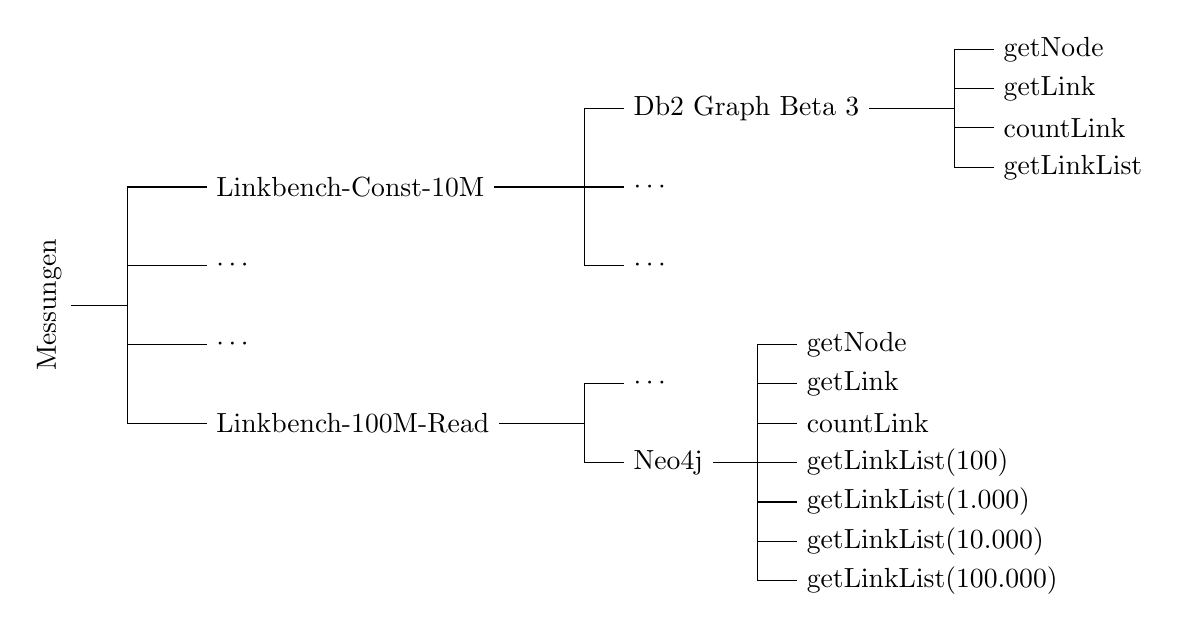
\begin{tikzpicture}
		\node[rotate=90] (messungen) at (0, 0) {Messungen};
		
		\node[anchor=west] (const) at (2, 1.5) {Linkbench-Const-10M};
		\draw (const.west) -- +(-1, 0) |- (messungen.south);
		\node[anchor=west] (p1) at (2, 0.5) {$\cdots$};
		\draw (p1.west) -- +(-1, 0) |- (messungen.south);
		\node[anchor=west] (p3) at (2, -0.5) {$\cdots$};
		\draw (p3.west) -- +(-1, 0) |- (messungen.south);
		\node[anchor=west] (read) at (2, -1.5) {Linkbench-100M-Read};
		\draw (read.west) -- +(-1, 0) |- (messungen.south);
		
		\node[anchor=west] (db2) at (7.3, 2.5) {Db2 Graph Beta 3};
		\draw (db2.west) -- +(-0.5, 0) |- (const.east);
		\node[anchor=west] (p11) at (7.3, 1.5) {$\cdots$};
		\draw (p11.west) -- +(-0.5, 0) |- (const.east);
		\node[anchor=west] (p12) at (7.3, 0.5) {$\cdots$};
		\draw (p12.west) -- +(-0.5, 0) |- (const.east);
		\node[anchor=west] (db2gn) at (12, 3.25) {getNode};
		\draw (db2gn.west) -- +(-0.5, 0) |- (db2.east);
		\node[anchor=west] (db2gl) at (12, 2.75) {getLink};
		\draw (db2gl.west) -- +(-0.5, 0) |- (db2.east);
		\node[anchor=west] (db2cl) at (12, 2.25) {countLink};
		\draw (db2cl.west) -- +(-0.5, 0) |- (db2.east);
		\node[anchor=west] (db2gll) at (12, 1.75) {getLinkList};
		\draw (db2gll.west) -- +(-0.5, 0) |- (db2.east);
		
		\node[anchor=west] (p21) at (7.3, -1.0) {$\cdots$};
		\draw (p21.west) -- +(-0.5, 0) |- (read.east);
		\node[anchor=west] (neo4j) at (7.3, -2.0) {Neo4j};
		\draw (neo4j.west) -- +(-0.5, 0) |- (read.east);
		\node[anchor=west] (n4jgn) at (9.5, -0.5) {getNode};
		\draw (n4jgn.west) -- +(-0.5, 0) |- (neo4j.east);
		\node[anchor=west] (n4jgl) at (9.5, -1.0) {getLink};
		\draw (n4jgl.west) -- +(-0.5, 0) |- (neo4j.east);
		\node[anchor=west] (n4jcl) at (9.5, -1.5) {countLink};
		\draw (n4jcl.west) -- +(-0.5, 0) |- (neo4j.east);
		\node[anchor=west] (n4jgll100) at (9.5, -2.0) {getLinkList(100)};
		\draw (n4jgll100.west) -- +(-0.5, 0) |- (neo4j.east);
		\node[anchor=west] (n4jgll1000) at (9.5, -2.5) {getLinkList(1.000)};
		\draw (n4jgll1000.west) -- +(-0.5, 0) |- (neo4j.east);
		\node[anchor=west] (n4jgll10000) at (9.5, -3.0) {getLinkList(10.000)};
		\draw (n4jgll10000.west) -- +(-0.5, 0) |- (neo4j.east);
		\node[anchor=west] (n4jgll100000) at (9.5, -3.5) {getLinkList(100.000)};
		\draw (n4jgll100000.west) -- +(-0.5, 0) |- (neo4j.east);
	\end{tikzpicture}
    \caption{Gliederung der Messungen}
    \label{fig:gliederung_messungen}
\end{figure}